\documentclass[a4paper,12pt]{article}
\usepackage[utf8]{inputenc}
\usepackage[brazilian]{babel}
\usepackage{amsmath}
\usepackage{amsfonts}
\usepackage{amssymb}
\usepackage{enumitem}
\usepackage{geometry}
\usepackage{graphicx}
\usepackage{caption}

\geometry{margin=2.5cm}

\title{Lista de Exercícios 1: Teoria e Aplicação de Diodos}

\date{Março de 2026}

% Configura a legenda para ter o rótulo e o texto em negrito.
\captionsetup[figure]{font=bf}

\begin{document}

\maketitle

\section*{Formulário de Apoio}

Considere as seguintes constantes e equações fundamentais para a resolução:

\begin{itemize}
    \item \textbf{Equação de Shockley:} $I_D = I_s \left( e^{\frac{V_D}{n V_T}} - 1 \right)$
    \item \textbf{Tensão Térmica:} $V_T = \frac{k T}{q} \approx 26\text{ mV}$ (a $300\text{ K}$)
    \item \textbf{Conversão de Temperatura:} $T_K = T_C + 273$
    \item \textbf{Potência no Zener:} $P_Z = V_Z I_Z$
    \item \textbf{Relações no Regulador Zener:}
    \begin{itemize}
        \item $I_R = I_Z + I_L$
        \item $V_R = V_i - V_L$
        \item $I_R = \frac{V_i - V_Z}{R_s}$
    \end{itemize}
\end{itemize}

\hrule
\section*{Questões Selecionadas}

\begin{enumerate}[label=\textbf{Questão \arabic*:}]

    % --- PARTE 1: SHOCKLEY E TEMPERATURA ---
    
    \item \textbf{a)} Determine a tensão térmica ($V_T$) de um diodo a uma temperatura de $20~^\circ\text{C}$.
    \par \textbf{b)} Para o mesmo diodo, determine a corrente $I_D$ usando a Equação de Shockley, dados $I_s = 40\text{ nA}$, $n = 2$ e $V_D = 0,5\text{ V}$.

    \item Repita a questão anterior considerando $T = 100~^\circ\text{C}$ e que a corrente de saturação reversa aumentou para $I_s = 5,0~\mu\text{A}$.

    \item Determine a corrente de diodo a $20~^\circ\text{C}$ para um diodo de silício ($n = 2$, $I_s = 0,1~\mu\text{A}$) sob polarização reversa de $-10\text{ V}$. O resultado condiz com o modelo ideal?

    \item Com $I_D = 8\text{ mA}$, $n = 1$ e $T = 25~^\circ\text{C}$, determine o valor da corrente de saturação reversa ($I_s$) para uma tensão aplicada de $0,5\text{ V}$.

    \item Se $I_D = 6\text{ mA}$, $V_T = 26\text{ mV}$, $n = 1$ e $I_s = 1\text{ nA}$, qual é a tensão $V_D$ aplicada ao diodo?

    \item A corrente de saturação de um diodo de silício é $0,1~\mu\text{A}$ a $20~^\circ\text{C}$. Determine seu valor aproximado se a temperatura ambiente subir $40~^\circ\text{C}$.

    % --- PARTE 2: PROJETOS ZENER ---

    \item Para o circuito da Figura 2.186, determine $V_L, I_L, I_Z$ e $I_R$ considerando:
    \begin{enumerate}[label=\alph*)]
        \item $R_L = 180~\Omega$.
        \item $R_L = 470~\Omega$.
        \item O valor de $R_L$ que estabelece a potência máxima no Zener.
    \end{enumerate}
    
    \begin{figure}[htbp]
        \centering
        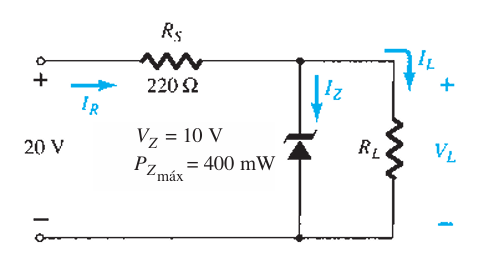
\includegraphics[width=0.8\textwidth]{2.186.png}
        \caption{Circuito Regulador Zener - Figura 2.186 do livro Boylestad.}
        \label{fig:2.186}
    \end{figure}

    \item Projete o circuito da Figura 2.187 para manter $V_L = 12\text{ V}$ com variação de carga ($I_L$) entre $0$ e $200\text{ mA}$. Determine $R_s$, $V_Z$ e a potência $P_{Zmax}$.
    \begin{figure}[htbp]
        \centering
        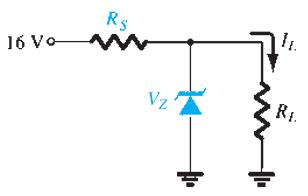
\includegraphics[width=0.7\textwidth]{2.187.png}
        \caption{Circuito Regulador Zener - Figura 2.187 do livro Boylestad.}
        \label{fig:2.187}
    \end{figure}

    \item Para o circuito da Figura 2.188, determine a faixa de valores de $V_i$ que manterá a saída $V_L$ regulada em $8\text{ V}$ sem exceder a potência nominal do diodo Zener.
    \begin{figure}[htbp]
        \centering
        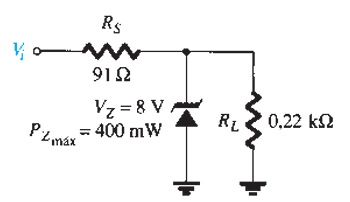
\includegraphics[width=0.8\textwidth]{2.188.png}
        \caption{Circuito Regulador Zener - Figura 2.188 do livro Boylestad.}
        \label{fig:2.188}
    \end{figure}

    \item Projete um regulador para $V_{out} = 20\text{ V}$ com carga de $1\text{ k}\Omega$, onde a entrada varia entre $30\text{ V}$ e $50\text{ V}$. Defina $R_s$ e a corrente máxima $I_{ZM}$.

\end{enumerate}

\newpage
\section*{Gabarito Detalhado: Análise e Resolução}

\begin{enumerate}[label=\textbf{Questão \arabic*:}, leftmargin=*]

    % --- Questão 1 ---
    \item \textbf{Análise de Sensibilidade Térmica}
    \begin{itemize}
        \item \textbf{a)} $T_K = 20 + 273 = 293\text{ K} \implies V_T = \frac{1,38 \times 10^{-23} \cdot 293}{1,6 \times 10^{-19}} \approx \mathbf{25,27\text{ mV}}$.
        \item \textbf{b)} $I_D = 40\text{ nA} \cdot (e^{0,5/(2 \cdot 0,02527)} - 1) \approx \mathbf{789,24~\mu\text{A}}$.
        \item \textit{Insight:} Note que a tensão térmica $V_T$ define a inclinação da curva característica do diodo; pequenas variações na temperatura alteram significativamente a condução.
    \end{itemize}

    % --- Questão 2 ---
    \item \textbf{Efeito do Aquecimento na Condução}
    \begin{itemize}
        \item $T_K = 373\text{ K} \implies V_T \approx 32,17\text{ mV}$.
        \item $I_D = 5~\mu\text{A} \cdot (e^{0,5/(2 \cdot 0,03217)} - 1) \approx \mathbf{11,83\text{ mA}}$.
        \item \textbf{Comentário:} O aumento da temperatura elevou a corrente em ordem de magnitude, evidenciando o coeficiente negativo de temperatura dos semicondutores.
    \end{itemize}

    % --- Questão 3 ---
    \item \textbf{Polarização Reversa e Modelagem}
    \begin{itemize}
        \item $V_D = -10\text{ V} \implies e^{V_D/nV_T} \ll 1 \implies I_D \approx -I_s = \mathbf{-0,1~\mu\text{A}}$.
        \item \textbf{Análise:} Diferente do modelo ideal ($I_{rev} = 0$), o modelo de Shockley prevê a corrente de saturação reversa, crucial para projetos de baixa potência.
    \end{itemize}

    % --- Questão 4 ---
    \item \textbf{Extração de Parâmetros: Corrente de Saturação}
    \begin{itemize}
        \item $I_s = \frac{I_D}{e^{V_D/nV_T} - 1} = \frac{8\text{ mA}}{e^{0,5/0,026} - 1} \approx \mathbf{35,7\text{ pA}}$.
        \item \textit{Nota:} Este valor extremamente baixo de $I_s$ é típico de diodos de silício modernos em temperatura ambiente.
    \end{itemize}

    % --- Questão 5 ---
    \item \textbf{Cálculo da Tensão de Barreira ($V_D$)}
    \begin{itemize}
        \item $V_D = nV_T \ln\left(\frac{I_D}{I_s} + 1\right) = 26\text{ mV} \cdot \ln\left(\frac{6\text{ mA}}{1\text{ nA}} + 1\right) \approx \mathbf{0,405\text{ V}}$.
    \end{itemize}

    % --- Questão 6 ---
    \item \textbf{Regra Prática de Temperatura}
    \begin{itemize}
        \item Para cada $10~^\circ\text{C}$ de aumento, $I_s$ aproximadamente dobra.
        \item $\Delta T = 40~^\circ\text{C} \implies 4 \text{ dobros} \implies I_{s,novo} = 0,1~\mu\text{A} \cdot 2^4 = \mathbf{1,6~\mu\text{A}}$.
    \end{itemize}

    % --- Questão 7 ---
    \item \textbf{Análise do Regulador Zener (Figura 2.186)}
    \begin{itemize}
        \item \textbf{a)} Divisor de tensão: $V_{Th} = 20 \cdot \frac{180}{400} = 9\text{ V}$. Como $V_{Th} < V_Z$, o Zener está em \textbf{corte (OFF)}. Logo, $V_L = V_{Th} = \mathbf{9\text{ V}}$ e $I_Z = \mathbf{0}$.
        \item \textbf{b)} $V_{Th} = 20 \cdot \frac{470}{690} \approx 13,6\text{ V} > V_Z$. Zener em \textbf{condução (ON)}. $V_L = V_Z = \mathbf{10\text{ V}}$.
        \item Correntes: $I_R = \frac{20-10}{220} \approx 45,5\text{ mA}$; $I_L = \frac{10}{470} \approx 21,3\text{ mA} \implies I_Z = I_R - I_L = \mathbf{24,2\text{ mA}}$.
        \item \textbf{c)} Para $P_{Zmax} = 400\text{ mW} \implies I_{Zmax} = 40\text{ mA}$. $I_{Lmin} = I_R - I_{Zmax} = 5,5\text{ mA} \implies R_{Lmax} \approx \mathbf{1818~\Omega}$.
    \end{itemize}

    % --- Questão 8 ---
    \item \textbf{Projeto de Regulador para Carga Variável}
    \begin{itemize}
        \item Para manter $V_L=12\text{ V}$, fixamos $V_Z = \mathbf{12\text{ V}}$.
        \item $R_s = \frac{V_i - V_Z}{I_{Lmax}} = \frac{16-12}{200\text{ mA}} = \mathbf{20~\Omega}$.
        \item $P_{Zmax} = V_Z \cdot I_{R} = 12\text{ V} \cdot 200\text{ mA} = \mathbf{2,4\text{ W}}$.
    \end{itemize}

    % --- Questão 9 ---
    \item \textbf{Faixa de Operação da Tensão de Entrada (Figura 2.188)}
    \begin{itemize}
        \item $I_L = 8\text{ V}/220~\Omega \approx 36,36\text{ mA}$.
        \item $V_{i,min} = 8 + (36,36\text{mA} \cdot 91) \approx \mathbf{11,31\text{ V}}$.
        \item $I_{Zmax} = 50\text{ mA} \implies I_{Rmax} = 86,36\text{ mA} \implies V_{i,max} = 8 + (86,36\text{mA} \cdot 91) \approx \mathbf{15,86\text{ V}}$.
    \end{itemize}

    % --- Questão 10 ---
    \item \textbf{Dimensionamento de Regulador sob Oscilação de Entrada}
    \begin{itemize}
        \item Carga: $I_L = 20\text{ V}/1\text{ k}\Omega = 20\text{ mA}$.
        \item Para garantir regulação em $V_{i,min}=30\text{V}$: $R_s = \frac{30-20}{20\text{ mA}} = \mathbf{500~\Omega}$.
        \item Em $V_{i,max}=50\text{V}$: $I_{Rmax} = \frac{50-20}{500} = 60\text{ mA} \implies I_{ZM} = 60 - 20 = \mathbf{40\text{ mA}}$.
    \end{itemize}

\end{enumerate}
\end{document}
